%- datasets
%-- unimorph
%-- bibles corpus?
%-- celex
%- permute phonemes
%- permute syllables
%- permute phonemes only within syllables
%- permute morphemes 
%\section{Morphology}

The memory--surprisal trade-off described in Section~\ref{sec:ms-tradeoff} should apply not just at the level of words, but at the level of any linguistic element. For instance, just as observed word orders exhibit information locality, the order of morphemes within words should also be structured so that morphemes which predict each other are close to each other.\jd{you haven't been talking about things in terms of information locality in the previous 2 sections, so this is surprising here. perhaps emphasize towards the end of the previous section again how we see information locality  in the results, then readers will be ready to think about this for morpheme order as well}

Here, we apply the memory--surprisal trade-off to explain \jd{"explain" is strong -- perhaps instead "predict"?} the order of morphemes within morphologically complex words in two agglutinative languages. We study two agglutinative languages for which extensive corpora with hand-annotated morphological segmentation and labeling are available: Japanese and Sesotho. Below, we give brief sketches of the morphological patterns in these languages. 

\jd{before going into the languages and then immediately diving into the methodological details, give the reader a broad outline of what will happen in this section -- what is the general procedure and argument at an abstract level?}


\paragraph{Verb Suffixes in Japanese}

In Japanese, verbs are marked with an extensive number of suffixes. For example, the following verb forms are marked with multiple suffixes:

\ex.\ag. mi  rare mash yoo \\
%Stem (3) (5) (8) \\
see  \textsc{passive}  \textsc{politeness}  \textsc{future} \\
`will be seen'
\bg. mi taku nakat ta \\
%Stem (6) (7) (8) \\
see \textsc{desiderative} \textsc{negation} \textsc{past} \\
`did not wish to see'

Based on corpus data and the linguistic literature on Japanese, we identified the following frequent verb suffixes, occurring in the following order outwards from the verb root (see SI for details).


\begin{enumerate}
\item \textit{suru}: obligatory suffix after Sino-Japanese words when they are used as verbs
\item Valence: causative (-\textit{ase}-) (\citet[142]{hasegawa2014japanese}, \citet[Chapter 13]{kaiser2013japanese})
\item Voice: passive (-\textit{are}-, -\textit{rare}-) \cite[152]{hasegawa2014japanese} \cite[Chapter 12]{kaiser2013japanese}
\item Mood: potential (-\textit{e}-, -\textit{are}-, -\textit{rare}-) \cite[398]{kaiser2013japanese}  
\item Politeness (-\textit{mas}-) \cite[190]{kaiser2013japanese}.
\item Mood: desiderative (-\textit{ta}-) \cite[238]{kaiser2013japanese}
\item Negation (-\textit{n}-)
\item Tense/Aspect/Mood/Finiteness: past (-\textit{ta}), future/hortative (-\textit{yoo}) \cite[229]{kaiser2013japanese}, nonfiniteness (-\textit{te}) \cite[186]{kaiser2013japanese}
%\item Nonfiniteness: the suffix -\textit{te} derives a nonfinite form .
\end{enumerate}

%In accordance with Bybee's hierarchy, valence is marked closest to the verb, followed by voice.
%Unlike predicted by the hierarchy, tense/aspect markers are not placed closer to the verb than mood/modality markers.






\paragraph{Verb Affixes in Sesotho}
Sesotho (also known as Southern Sotho) is a Southern Bantu language spoken primarily in Lesotho and South Africa.
Sesotho verbs are marked with both prefixes and suffixes.
Common prefixes include markers for agreement with subjects and objects; object prefixes always follow subject prefixes \ref{ex:oadireka}.
Common suffixes include markers changing valence and voice, and a mood suffix \ref{ex:ophehela}.

\ex.\ag. oa di rek a \\
\textsc{subject.agreement} \textsc{object.agreement} buy \textsc{indicative} \\
`(he) is buying (it)'  \cite[ex (41)]{demuth1992acquisition} \label{ex:oadireka}
\bg. o pheh el a \\
\textsc{subject.agreement} cook \textsc{applicative} \textsc{indicative} \\
`(he) cooks (food) for (him)'  \cite[ex (41)]{demuth1992acquisition}
\label{ex:ophehela}

We identified affix morphemes and their ordering based on the analysis in \cite{demuth1992acquisition}, supplemented with information from grammars of Sesotho \citep{doke1967textbook,guma1971outline}. See SI for details.
We identified the following prefixes:

\begin{enumerate}
    \item Subject agreement: This morpheme encodes agreement with the subject, for person, number, and noun class (the latter only in the 3rd person) \cite[\textsection 395]{doke1967textbook}.
	    The annotation provided by \cite{demuth1992acquisition} distinguishes between ordinary subject agreement prefixes and agreement prefixes used in relative clauses; we distinguish these morpheme types here.
    
    \item Negation \cite[\textsection 429]{doke1967textbook}
    
    \item Tense/aspect marker   \cite[\textsection 400--424]{doke1967textbook}
    
    \item Object agreement or reflexive marker \cite[\textsection 459]{doke1967textbook}. 
    Similar to subject agreement, object agreement denotes person, number, and noun class features of the object.
\end{enumerate}
We identified the following suffixes:

% something we might cite at some point (pointers from Beth Levine), about templatic morpheme order in Bantu
% Hyman2003 in literature.bib
% Jeffrey Good, Strong Linearity: Three Case Studies Towards a Theory of Morphosyntactic Templatic Constructions (Diss, 2003)
    
\begin{enumerate}
\item Semantic derivation: reversive (e.g., `do' $\rightarrow$ `undo') \cite[\textsection 345]{doke1967textbook}
\item Valence: Common valence-altering suffixes include causative, neuter/stative, applicative, and reciprocal \cite[\textsection 307--338]{doke1967textbook}. See SI for details on their meanings.
    \item Voice: passive \cite[\textsection 300]{doke1967textbook} 
    \item Tense \cite[\textsection 369]{doke1967textbook}
    \item Mood \cite[\textsection 386--445]{doke1967textbook}
    \item Interrogative and relative markers, appended to verbs in certain interrogative and relative clauses \cite[\textsection 160, 271, 320, 714, 793]{doke1967textbook}.
    %-\textit{ng}.
    %The interrogative marker -\textit{ng} is an enclitized form of the interrogative `what'.
    %The relative marker -\textit{ng} is suffixed to verbs in relative clauses.
\end{enumerate}



%For prefixes, in agreement with Bybee's hierarchy, subject agreement is encoded in a position further away than TAM features.
%For suffixes, relation to Bybee hierarchy: valence closest, then voice, then tense, then mood.


\subsection{Experiment}
\paragraph{Data Selection and Processing}
\jd{none of this makes any sense to the reader if you don't say first what the general approach looks like for the work reported in this section (see comment above)} For Japanese, we drew on Universal Dependencies data.
In the tokenization scheme used for Japanese, most affixes are separated as individual tokens, effectively providing morpheme segmentations.
We used the GSD corpus, Version 2.4, \citep{tanaka2016universal, asahara2018universal}, as it was the only corpus with a training set and freely available word forms.
In the corpus, verb suffixes largely correspond to auxiliaries (with tag \texttt{AUX}); only a few morphemes tagged \texttt{AUX} are not standardly treated as suffixes (see SI), and one frequent suffix (-\textit{te}) is labeled \texttt{SCONJ}.
We selected verb forms by selecting all chains of a verb (tag \texttt{VERB}) followed by any number of auxiliaries (tag \texttt{AUX}) from the training set of the corpus. When the suffix -\textit{te} (tag \texttt{SCONJ}) followed such a chain, we added this.
We labeled suffixes for underlying morphemes with the help of the lemmatization provided for each suffix in the corpus (see SI for details).
We obtained 15,281 verb forms in the training set and 1,048 verb forms in the held-out set.
Of the forms in the training set, 27\% had two or more suffixes (modal group: two suffixes, 20\%\jd{what does this 20\% mean? perhaps provide plot of distribution over number of suffixes (in SI)? }; maximum seven suffixes).
While predicting order naturally focuses on datapoints with more than one suffix, we include the other datapoints for estimating conditional mutual information $I_t$.
%We used the annotation provided in the corpus to identify underlying morphemes (see SI).

%In the corpus, each morpheme is annotated with a lemma, indicating a normalized context-independent representation of the morpheme.
%For both verbs and affixes, this lemma annotation abstracts away from most morphophonological and other allomorphic variation, it thus largely identifies underlying morphemes (see SI for limitations).

For Sesotho, we used the Demuth Corpus \citep{demuth1992acquisition} of child and child-directed speech, containing about 13K utterances with 500K morphemes.
The corpus has very extensive manual morphological segmentation and annotation; each verb form is segmented into morphemes, which are annotated for their function.
Sesotho verbs carry both prefixes and suffixes.
We extracted 37K verb forms (see SI for details).
We randomly selected 5\% to serve as held-out data and used the remaining 95\% as training data.
93\% of forms had two or more affixes (modal group: three affixes, 36\%; maximum eight affixes).


\paragraph{Estimating Memory-Surprisal Tradeoff}
We model predicted morpheme sequences.
To do so, we represent each verb form as a sequence of a stem and suffix morphemes, abstracting away from morphophonemic interactions between neighboring morphemes.\jd{is it possible that, where there is divergence between model predictions and actual order, it has sth to do with phonemic pressures?}
As in many languages, affixes in Japanese and Sesotho show morphophonemic interactions between neighboring morphemes; for instance, the Japanese politeness morpheme -\textit{mas}- takes the form -\textit{masu} when it is word-final, while it has the allomorph -\textit{mase}- when followed by the negation suffix -\textit{n}.
Modeling prediction on the level of morphemes, as opposed to phonemes, controls for these interactions.\footnote{See SI Section \REF for qualitatively similar results when modeling prediction at the phoneme level.}


We model verb forms as a stochastic process by concatenating the verb forms from the corpus in random order.
This means, we model statistical dependencies between the different morphemes in a form, and no dependencies between verb forms and their surrounding words. \jd{i don't know what this is supposed to mean.}

We calculate $I_t$ by estimating an $n$-gram model on the training set and then computing the average surprisal $S_t$ as cross-entropy on the held-out set using Kneser-Ney smoothing.
The model may overfit as the context size $t$ increases, leading to higher cross-entropies for larger values of $t$.
To mitigate this problem, we estimate
\begin{equation}
\hat{S}_t := \min_{s \leq t} S_s,
\end{equation}
where $S_s$ is the cross-entropy of the $s$'th order Markov model on held-out data.
This procedure ensures that $\hat{S}_t$ can only decrease as the context size $t$ increases.
Similar results are obtained when instead using the simple `naive' estimator for $I_t$ on the training set; see the SI for details.

\paragraph{Parameterizing Alternative Orderings}

We parameterize alternative affix orderings by assigning a weight in $[0,1]$ to each morpheme.
Given such a grammar, affixes are ordered by the values assigned to their underlying morphemes.
We consider all morphemes annotated in the corpora, including low-frequency ones going beyond the ones identified above (see SI for details).

In Japanese, the passive (slot 3) and potential (slot 4) markers are formally indistinguishable for many verbs.
As we cannot systematically distinguish them on the basis of the available corpus annotation, we merge these into a single underlying morpheme `Passive/Potential'.\jd{this is a detail that should come earlier, in the data selection/processing subsection}


To verify that this formalism is appropriate for capturing morpheme order in Japanese and Sesotho, we fitted models parameterized in this way to the observed orders.
Ordering morphemes according to these fitted models recovered the observed order for almost all forms (98.6 \% for Japanese, 99.93\% for Sesotho prefixes, 97.4\% for Sesotho suffixes). Exceptions largely concern low-frequency affixes beyond those considered here. We take this as confirmation that the formalism is generally suited to capture morpheme order.


\paragraph{Creating Optimal Orders}

In order to create optimal orders to compare real orders to, we optimize orderings for the AUC under the memory-surprisal tradeoff curve with an adaptation of the hill climbing method used by \citet{gildea-human-2015} to optimize word order grammars for the length of syntactic dependencies and trigram surprisal.

We randomly initialize the assignment of weights to morphemes, and then iteratively change the assignment to reduce AUC.
In each iteration, we randomly choose one morpheme, and evaluate AUC for each way of ordering it between two other morphemes.
We then update the weights to the ordering that yields the lowest AUC.
To speed up optimization, we restrict to morphemes occurring at least 10 times in the corpus for 95\% of iterations, and to 10\% of possible orderings in each step.
These choices vastly reduce computation time by reducing time spent on low-frequency morphemes.
This optimization method is approximate, as it only guarantees convergence to a local optimum, not to a globally optimal assignment.

We ran this method for 1,000 iterations. Empirically, AUC converges after a few hundred iterations.
To control for the randomness in initialization and the optimization steps, we ran this algorithm ten times. \jd{so you can put error bars on the optimized order data point in figure 19 (the AUC plot)?}
For Sesotho, we ran the algorithm separately for prefixes and suffixes.\jd{if you don't run it separately, does it not work?}

\subsection{Results}
In Figure~\ref{fig:morph-auc}, we compare the area under curve of the memory--surprisal trade-off for Japanese and Sesotho verb forms under different orderings.
Both observed orders and the approximately optimized grammars show lower AUCs than all random baseline samples.
For comparison, we also show AUC for the order resulting from \emph{reversing} all suffix chains in the observed orders; this results in high AUC even exceeding most random grammars.
These results show that Japanese and Sesotho affix orderings enable approximately optimal memory-surprisal tradeoffs.



\begin{figure}
	\begin{center}
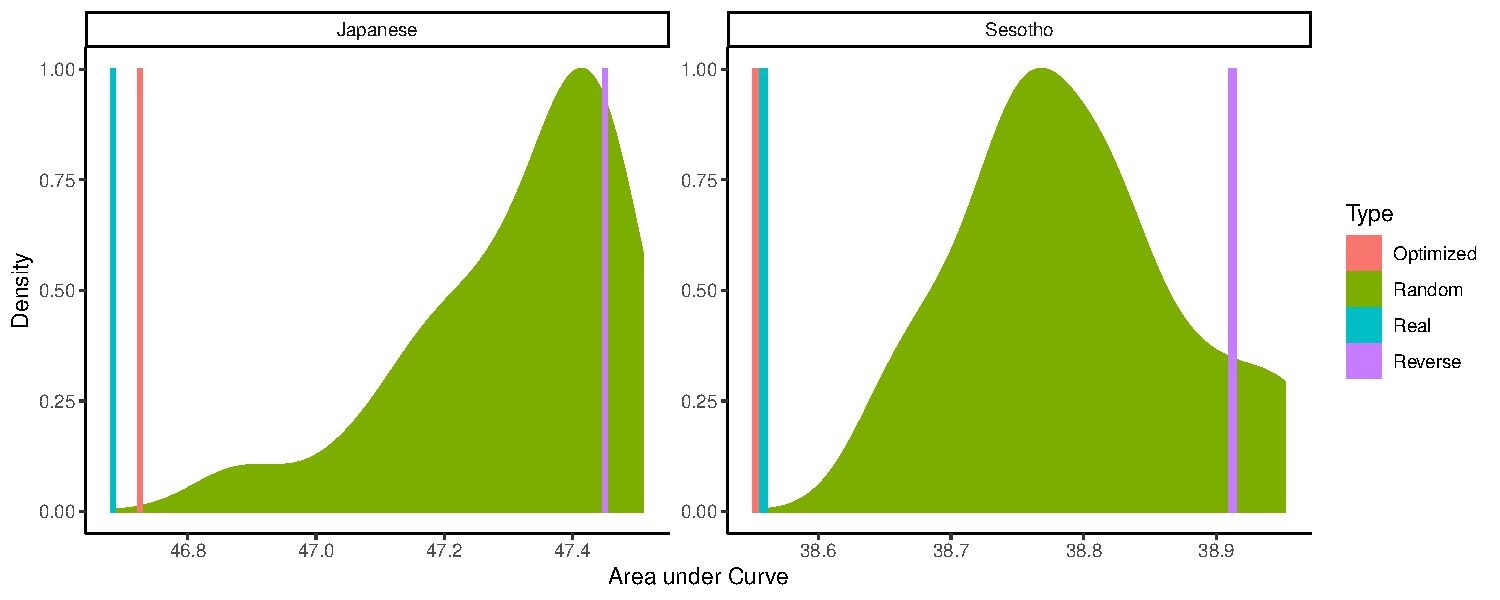
\includegraphics[width=\textwidth]{figures/Both-suffixes-byMorphemes-auc-hist-heldout.pdf}
\end{center}
	\caption{Areas under the curve for the memory-surprisal tradeoff for verb affixes in Japanese (left) and Sesotho (right). \mhahn{make numbers larger} \jd{i think i've asked this before, but how can the real language be better than the optimized one(s)? is it because the optimized versions sometimes get stuck in local optima? this is where it would be useful to get error bars on the optimized AUCs}}
	\label{fig:morph-auc}
\end{figure}



%\begin{figure}
%	\begin{center}
%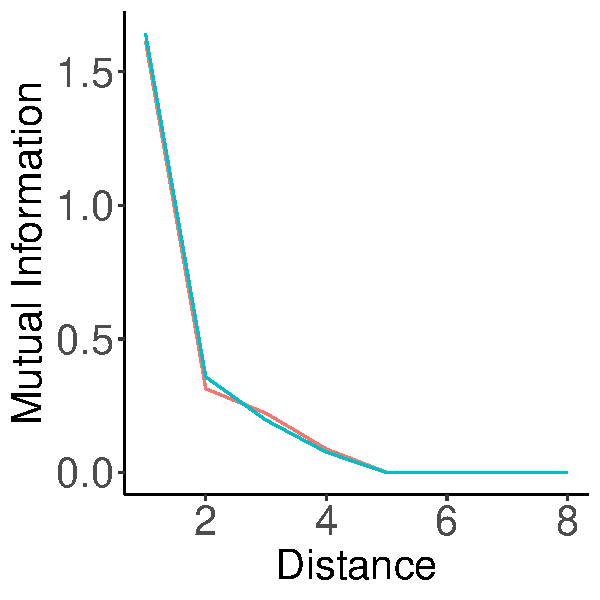
\includegraphics[width=0.3\textwidth]{figures/Japanese-suffixes-byPhonemes-it-heldout.pdf}
%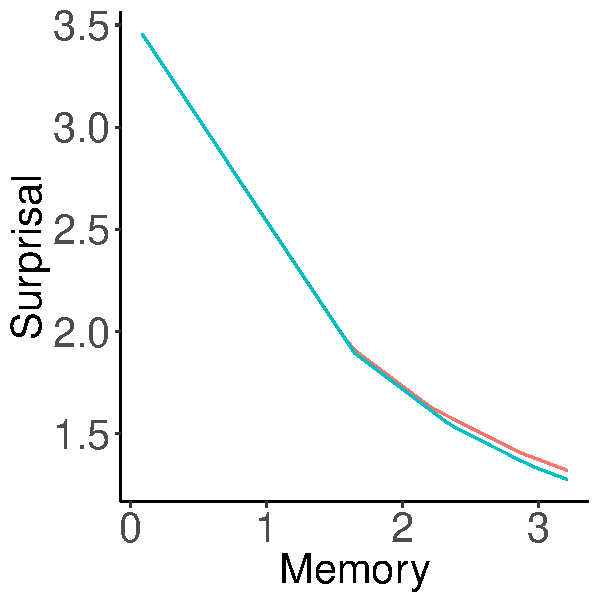
\includegraphics[width=0.3\textwidth]{figures/Japanese-suffixes-byPhonemes-memsurp-heldout.pdf}
%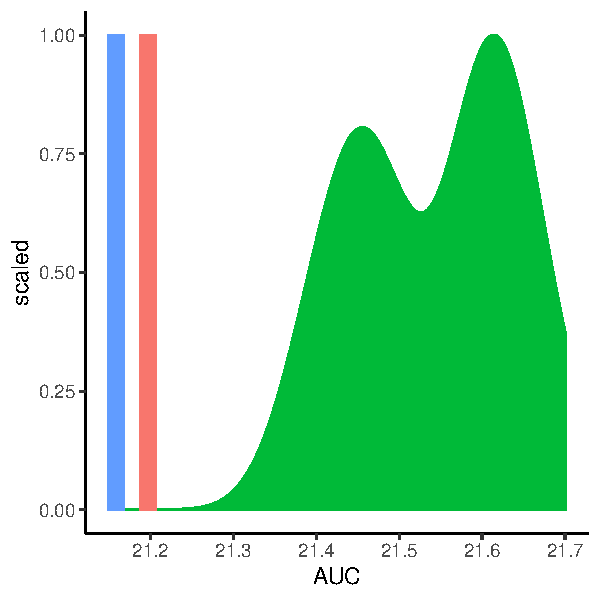
\includegraphics[width=0.3\textwidth]{figures/Japanese-suffixes-byPhonemes-auc-hist-heldout.pdf}
%
%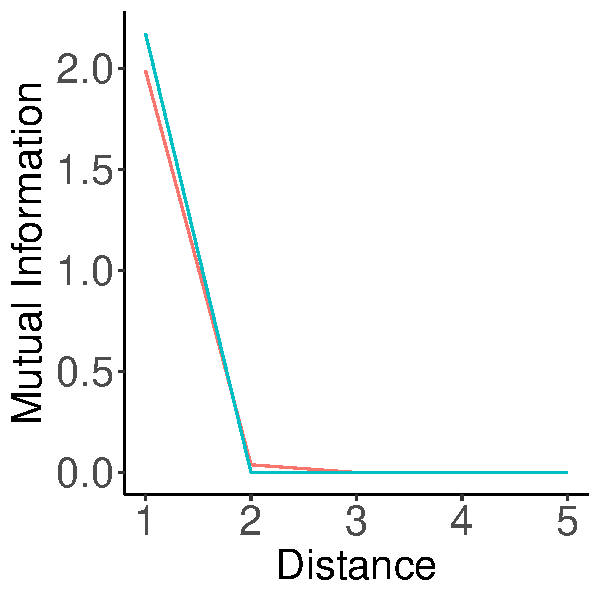
\includegraphics[width=0.3\textwidth]{figures/Japanese-suffixes-byMorphemes-it-heldout.pdf}
%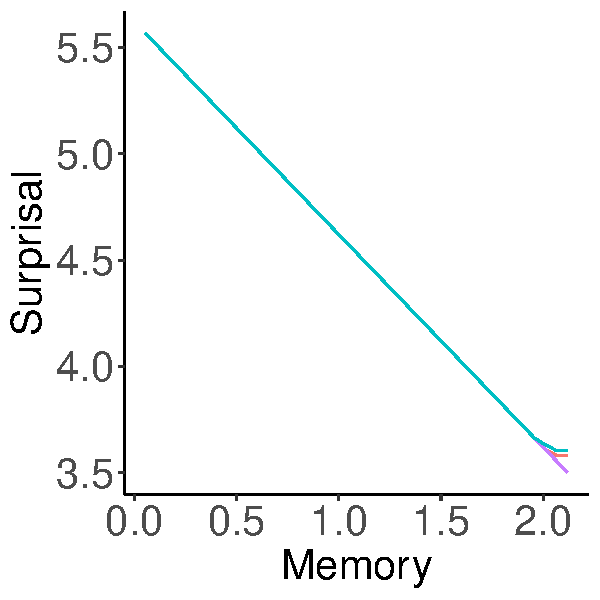
\includegraphics[width=0.3\textwidth]{figures/Japanese-suffixes-byMorphemes-memsurp-heldout.pdf}
%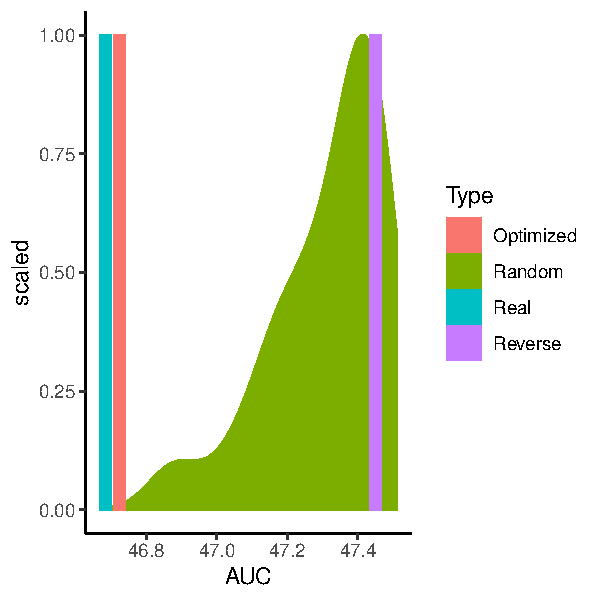
\includegraphics[width=0.3\textwidth]{figures/Japanese-suffixes-byMorphemes-auc-hist-heldout.pdf}
%\end{center}
%	\caption{Areas under the memory-surprisal tradeoff curve for Japanese verb suffixes.}\label{fig:jap-phon-morph}
	%\caption{Japanese verb suffixes, measuring prediction on the level of phonemes (top) and morphemes (bottom), for real (blue), random (green), and approximately optimized (red) orderings. Left: $I_t$ as a function of $t$. Center: Memory-surprisal tradeoff. Right: Areas under the curve for the memory-surprisal tradeoff.}\label{fig:jap-phon-morph}
%\end{figure}


We now ask to what extent the observed morpheme ordering is predicted correctly by approximately optimized grammars.
In Table~\ref{tab:morph-acc}, we give summary statistics about the accuracy of optimized grammars in predicting affix order in the corpus, together with random baseline figures.
We evaluate accuracy using two methods:
In one method (`Pairs'), we consider, for each verb form in the corpus, all pairs of prefixes (or suffixes).
We report the proportion of these pairs in the corpus for which the relative order of the two affixes is as predicted by the grammar.
In the other method, (`Full'), we report the proportion of verb forms in the corpus that has exactly the affix ordering predicted by the grammar.

\begin{table}
\begin{tabular}{cc||ll|ll}
             &              & \multicolumn{2}{c}{Prefixes}    & \multicolumn{2}{|c}{Suffixes} \\
             &              & Pairs & Full & Pairs & Full \\ \hline\hline
Japanese & Optimized  & -- &  -- &   0.954 (SD 0.009) & 0.945 (SD 0.012) \\ 
& Baseline    & -- & -- & 0.504 (SD 0.0) & 0.414 (SD 0.0) \\ \hline
%Phon.   &   Optimized  &  0.993 (SD 0.0) & 0.989 (SD 0.0) & 0.792 (SD 0.102) & 0.734 (SD 0.13) \\
%	& Random  &  0.322 (SD 0.253) & 0.195 (SD 0.24) & 0.588 (SD 0.155) & 0.554 (SD 0.167) \\ \hline
Sesotho &   Optimized  &  0.988 (SD 0.0) & 0.989 (SD 0.0) & 0.756 (SD 0.014) & 0.676 (SD 0.017) \\
&   Baseline  &  0.672 (SD 0.305) & 0.604 (SD 0.338) & 0.423 (SD 0.204) & 0.332 (SD 0.211) \\ 
\end{tabular}
\caption{Accuracy of approximately optimized orderings, and of random baseline orderings, in predicting verb affix order in Japanese and Sesotho. `Pairs' denotes the rate of pairs of morphemes that are ordered correctly, and `Full' denotes the rate of verb forms where order is predicted entirely correctly. We show means and standard deviations over different runs of the optimization algorithm (`Optimized'), and over different random orderings (`Random').}\label{tab:morph-acc}
\end{table}

\paragraph{Japanese results.} In Japanese, by both measures, optimized grammars recover the observed orders with high accuracy.
We compare the real grammar with the approximately optimized grammar that achieved the lowest AUC value in Table~\ref{tab:grammar-table-jap}; the main divergence is that desiderative suffixes are placed after the negation suffix (slot 6), whereas real Japanese orders place them before the politeness suffix (slot 5).

We conducted an error analysis comparing the real Japanese morpheme order against our approximately optimized orders.
For each grammar, we extracted the pairs of morphemes whose relative order is incorrectly predicted, excluding pairs involving low-frequency morphemes not discussed here. %, and including a few forms that do not agree with the dominant order described above (TODO figure out what these exceptions are).
Results are shown in Table~\ref{tab:jap-err-analysis}.
The most frequent divergence is that past and negation suffixes are consistently ordered incorrectly; this affects 88 corpus examples (out of 15K total examples).
%A few of the optimized grammars show additional divergences among high-frequency morphemes, for instance, some grammars order politeness and negation incorrectly. 

\begin{table}
    \centering
    \begin{tabular}{llllllll}
	    &	    Real & Optimized \\ \hline\hline
	    &    Stem & Stem \\ \hline
1 & suru & suru \\
2 & causative & causative \\
3 & passive/potential & passive/potential \\
4 & desiderative & desiderative \\
5 & politeness & future \\
6 & negation & politeness \\
7 & future & past \\
 & past & negation \\
 & nonfinite & nonfinite \\ 
 \hline
    \end{tabular}
    \caption{Comparing order of Japanese affixes in the observed orders (left) and according to an approximately optimized grammar (right).\jd{include the sesotho results as well (even if it doesn't look as clean). also, why do the numbers stop at 7?}}
    \label{tab:grammar-table-jap}
\end{table}

\begin{table}
    \centering
    \begin{tabular}{ll|ll}
    \multicolumn{2}{c|}{Error} & Frequency \\ \hline\hline
negation & past & 88 \\
politeness & future & 9 \\
%negation & suru & 6 \\
negation & politeness & 3 \\
%politeness & passive/potential & 2 \\
%causative & suru & 2 \\
\end{tabular}
    \caption{Errors in Japanese: We show pairs of morphemes that are ordered incorrectly by the approximately optimized grammar.
    We indicate the number of such pairs occurring in the corpus.
    We only count divergences as errors here if they are predicted by the order (TODO figure out where exceptions come from). Also, we only show errors where both morphemes are among the high-frequency ones studied here.
    %\rljf{How is the frequency column calculated?}
    }
    \label{tab:jap-err-analysis}
\end{table}

\paragraph{Sesotho results.} We compare the real Sesotho grammar with the approximately optimized grammar that achieved the lowest AUC value in Table~\ref{tab:grammar-table-sesotho}. \jd{hm, is it the case that the lowest-AUC optimized grammars differ in the predicted order? if so, that suggests further analyses} In Sesotho, for prefixes, all optimized grammars almost exactly recover the ordering described above.
The only divergence among the high-frequency morphemes is that negation and the tense/aspect prefix are ordered incorrectly; this accounts for only 12 occurrences in the data set, as the two prefixes rarely co-occur.
%Other divergences affect lower-frequency morphemes. % (TODO how many).
%Common divergences are shown in Table~\ref{tab:sesotho-prefix-err-analysis}.

For Sesotho suffixes, order is recovered at above-chance accuracies, though with some divergences.
The most common error (Table~\ref{tab:sesotho-prefix-err-analysis}) is that relative and interrogative suffixes are consistently placed closer to the verb stem than the mood suffix.
We conjecture that this happens because all Sesotho verbs uniformly have a mood suffix, suggesting that there might be lower mutual information between the stem and the mood suffix than between the stem and these two suffixes.
Furthermore, valence-changing suffixes are ordered farther away from the stem than various other suffixes, in contrast with the actual orders.
Interestingly, we found that prediction was more accurate in this respect when estimating $I_t$ naively \jd{when you first introduce the naive estimator above, say a little more about what that means} on the training set (see SI Figure \REF), suggesting that the available corpus data does not sufficiently determine the optimal ordering.

\begin{table}
    \centering
    \begin{tabular}{ll|ll}
    \multicolumn{2}{c|}{Error} & Frequency \\ \hline\hline
Negation & Tense/aspect & 12 \\
\\
    \multicolumn{2}{c|}{Error} & Frequency \\ \hline\hline
Mood & Interrogative & 2204 \\
Mood & Relative & 858 \\
Applicative & Tense/aspect & 347 \\
%Tense/aspect & Passive & 302 \\
Causative & Tense/aspect & 174 \\
Neuter & Tense/aspect & 155 \\
\end{tabular}
    \caption{Errors in Sesotho prefixes (top) and suffixes (bottom). We only count divergences as errors here if they are predicted by the order (TODO figure out where exceptions come from). Also, we only show errors where both morphemes are among the high-frequency ones studied here.}
    \label{tab:sesotho-prefix-err-analysis}
\end{table}




\begin{table}
    \centering
    \begin{tabular}{llllllll}
	    &	    Real & Optimized \\ \hline\hline
	    1 & Subject & Subject \\
	      & Subject (rel.) & Subject (rel.) \\
	    2 & Negation & Tense/aspect \\
	    3& Tense/aspect & Negation \\
	    4 &Object & Object \\ \hline
	    &Stem & Stem  \\ \hline
	    1 & Reversive & Passive \\
	    2& Causative & Reciprocal \\
	    &Neuter & Tense/aspect \\
	    &Applicative & Neuter \\
	    &Reciprocal & Relative \\
	    3&Passive & Causative \\
	    4&Tense/aspect & Applicative \\
	    5&Mood & Interrogative \\
	    6&Interrogative & Reversive \\
	    &Relative & Mood \\ \hline
    \end{tabular}
	\caption{Comparing order of Sesotho affixes in the observed orders (left) and according to an approximatively optimized grammar (right). Note that order was separately optimized for prefixes and suffixes.\jd{oh i see, you provide this table after all, just in the reverse order from what it is in the japanese section. make sure the orders are consistent, or just collapse the japanese and sesotho table into one}}
    \label{tab:grammar-table-sesotho}
\end{table}


%\begin{figure}
%\begin{center}
%\begin{tabular}{c||llll}
%             &       Pairs & Full \\ \hline\hline
%Optimized for Phoneme Prediction   &   0.962 (SD 0.001) & 0.957 (SD 0.002) \\
%Optimized  &   0.954 (SD 0.009) & 0.945 (SD 0.012) \\ 
%Random Baseline    &  0.504 (SD 0.0) & 0.414 (SD 0.0) \\ 
%\end{tabular}
%\end{center}
%\caption{Accuracy of approximately optimized orderings, and of random baseline orderings, in predicting verb suffix order in Japanese. `Pairs' denotes the rate of pairs of morphemes that are ordered correctly, and `Full' denotes the rate of verb forms where order is predicted entirely correctly. We show means and standard deviations over different runs of the optimization algorithm (`Optimized'), and over different random orderings (`Random').}\label{fig:acc-japanese}
%\end{figure}










\subsection{Discussion}
We have found that the ordering of verb affixes in Japanese and Sesotho provides approximately optimal memory--surprisal trade-offs. \jd{hm, that was more of a qualitative observation, wasn't it? if you put error bars on the optimized AUCs, could you argue that the real languages are approximately optimal because they fall within the 95\% CIs?}
We further found that parts of these languages' ordering rules can be derived from optimizing order for efficient tradeoffs.

We argue that the memory--surprisal trade-off provides an explanation of previously-existing typological generalizations, and an operationalization of previous functionally-motivated explanations for them.\jd{add a sentence here on why.}
Most prominently, \citet{bybee-morphology-1985} has claimed that a universal ordering of verbal inflectional morphemes exists across languages:
\begin{quote}
\begin{tabular}{llllllllllllllllllllllllll}
verb stem & valence & voice & aspect & tense& mood & modality & subj. person & subj.number 
\end{tabular}
\end{quote}
Morphemes are claimed either to go in the order above (suffixes), or its reverse (prefixes). This hierarchy makes no statements as to which affixes are realized as prefixes or suffixes.

Japanese and Sesotho verb affixes are broadly in agreement with Bybee's generalization.
For instance, valence and voice suffixes are closer to the stem than tense/aspect/mood markers.
Subject agreement in Sesotho is farther away from the verb than tense/aspect/mood prefixes.
This ordering is reproduced closely by optimization in Japanese and for Sesotho prefixes, and to some extent also for Sesotho suffixes.

\citet[p. 37]{bybee-morphology-1985} argues further that morpheme order is determined by the degree of \emph{relevance} between the affix and the stem, that is, the degree to which ``the semantic content of the first [element] directly affects or modifies the semantic content of the second'' (p. 13).
She argues that elements whose meanings are more relevant to each other appear closer together.
For instance, the meaning of a verb is impacted more strongly by a causative affix than by a tense affix:
Combining a verb with a causative marker results in a form that denotes a different action, whereas a tense affix only locates the action in time.

We conjecture that this notion of relevance is related to mutual information.
If an affix has a stronger impact on the meaning of the verb, it will typically not be applicable to all verbs.
For instance, causative markers will only attach to verbs whose semantics is compatible with causation.
In contrast, a past tense marker can attach to all verbs that are compatible with actions that can have occurred in the past.
Therefore, we expect that affixes that are more relevant to a verb stem will also tend to have higher mutual information with the verb stem.
If they have higher mutual information with the verb stem, then the principle of information locality predicts that they will go close to the verb stem.
